\documentclass[a4papert,11pt,notitlepage]{ltxdoc}
\usepackage[left=1.0in, right=1.0in, top=1.0in, bottom=1.0in]{geometry}
\usepackage[parfill]{parskip}
\usepackage{graphicx}
\usepackage{epstopdf}
\usepackage{mdwlist}
\usepackage{amssymb}
\usepackage{todonotes}
\usepackage{longtable}
\usepackage{fancyhdr}
\usepackage{appendix}
\pagestyle{fancy}

\DeclareGraphicsRule{.tif}{png}{.png}{`convert #1 `dirname #1`/`basename #1 .tif`.png}
\bibliographystyle{plain-annote}

\title{Developing a device-agnostic, real-time ARS/PRS system with support for
broadcasting rich interactive content}

\begin{document}
\vspace*{\fill}
\begin{center}
\textsc{\Large Final Major Project - Internet Engineering (H622)}\\[0.3cm]
{\Large \bfseries Developing a device-agnostic, real-time ARS/PRS system with support for
broadcasting rich interactive content}\\[0.3cm]
{\Large Final Report}\\[0.3cm]
\emph{Author:} Thomas \textsc{Usher} \hspace{1cm} \emph{Supervisor:} Dave \textsc{Price}\\
\emph{Date:} ---- \hspace{1cm} \emph{Version:} 0.1
\end{center}
\vspace*{\fill}
\pagebreak

\section*{Acknowledgements}
With thanks to Dave Price, for feedback, advice and suggestions to myself and the rest of the project group during the development of this project.

Many thanks to Denise Williams-Morris, Alex Kruzewski and my parents, for testing, feedback, proof-reading and moral support.

\listoftodos{}
\pagebreak

\section*{Abstract}
\todo[inline]{Some abstract}

\section*{Definition of Terms}
\begin{description}
\item[Presenter] \hfill \\
The user running a presentation. A lecturer, teacher or meeting co-ordinator.
\item[Attendee] \hfill \\
User attending a presentation. A student or one attending a meeting.
\item[Presentation] \hfill \\
A setting in which a single Presenter (occasionally multiple) is interacting with multiple Attendees, typically in order to present information. A lecture, class, talk or meeting.
\end{description}

\pagebreak

\tableofcontents

\pagebreak

\section{Background and Objectives}
\subsection{Context}
Audience Response Systems (ARS), more commonly referred to as `clickers' have been used with varying degrees of success in educational establishments around the world for numerous years. Their use as a means to improve interactivity between students and instructors in an educational environment has been widely documented, with research indicating notable effects on student responsiveness, involvement and success. 

From using these clickers from a students' perspective, three primary problem areas were noted with the current implementation of these ARS systems:
\begin{description}
\item[Accesibility] \hfill \\
Specific clicker hardware is required. While they can be relatively cheap, costs do increase with complexity and they are single-purposes devices. In most cases, specialist receiver hardware is also required and in larger scale cases, technicians are required to maintain these systems.
\item[Interaction] \hfill \\
The devices are limited in what can be displayed on an individual users' device - while the majority have no displays at all, those that do typically only show which number/letter the user has selected. This limitation restricts interaction to simple question and answer style communication, as well as limiting potential for individual or group specific broadcasts.
\item[Flexibility] \hfill \\
ARS devices are usually single-purpose and rarely used for anything beyond prompting an audience for answers to a question.
\end{description}

While this project does not involve additional research in to the value of ARS systems, it does attempt to highlight and enhance upon ``The give-and-take atmosphere encouraged by use of clickers which... makes the students more responsive in general''\cite{wood:clickers} while attempting to alleviate the above issues in a new, `evolved' ARS implementation.

\subsection{Objectives}
ARS' exist to improve interactivity during lectures, helping to engage students in the subject, improve attention-span and providing additional ways for students to feel personally involved in the presentation. Secondarily, facilitating real-time feedback allows lecturers to tailor their approach based on the class response - for example, the lecturer might broadcast a set of questions about the current topic, if a large percentage of students answer incorrectly, the lecturer might wish to attempt another explanation. 

This project attempts to maintain all of these benefits while creating a `next-generation' ARS system by focusing on improving the three problem areas: accessibility, interaction and flexibility:

\subsubsection{Accessibility}
\begin{itemize}
\item Improving ease and cost of setup/configuration for system administrators by leveraging existing local area networks, allowing the system to be configured once per site, rather than requiring setup for every presentation.
\item Facilitating ease of access by presenters by supporting the use of the presenter system on existing network-connected systems without the requirement for additional software installations.
\item Extending the use of ARS systems for attendees by using existing devices with a relatively modern web-browser and the ability to access the local network as clients. Allowing attendees to use their existing smartphones, tablets or laptops rather than using proprietary hardware.
\item Removing the requirement to have dedicated hardware installed and available when an ARS is required.
\item Simplifying the experience of interacting with the system for both the presenter and the attendee.
\end{itemize}

\subsubsection{Interaction}
By using the capabilities of powerful modern portable hardware, the system aims to provide multiple ways by which attendees can interact with the presenter during a presentation. While a typical ARS offers only Question and Answer style interaction, this system will allow a large variety of content to be broadcast and responded to, including images, puzzles and games.

As with standard ARS', the system is intended to facilitate near-instant, actionable feedback to the presenter from interactions with attendees.

\subsubsection{Flexibility}
Building the system around an extensible framework allows additional types of content to be created for broadcast by developers, creating infinite possible types of interaction supporting the use of system in many other use cases. By refraining from using any device-specific implementations/code, extending the system to support future devices should be trivial.

\subsection{Relevant Literature and Existing Systems}
A number of varying ARS systems were researched during project planning, full details on which can be found in Appendix \ref{app:existingars}. The general conclusion reached from this research was that all current ARS systems have not developed beyond the simple Question and Answer style interaction model, likely due to the restrictions of requiring legacy device support in their software.

\pagebreak

\section{Development Process}
\subsection{Process Model}
For this project, being able to enjoy the development of the system was important, so a process model which best suited the way the author wrote software needed to be adopted. As the author's typical development methodology is `hack at it until it works', a process model that injected a degree of organisation in to the process, providing a way to plan and view progress while maintaining focus on the code rather than the documentation needed to be found.

For this reason, the iterative development approach was chosen, as it best suits how the author builds software, allowing blocks of time in which the focus is on writing code, while adding a sense of organisation and planning to the process. While the waterfall model might also have been suitable, the requirement to complete the design before moving on to development was considered too restrictive as it is believed that any software project needs room to evolve during its implementation.

The iterative development model was adapted slightly to suit the project, following this cycle:
\begin{enumerate}
\item Produce overall specification document.
\item Begin iteration:
\begin{enumerate}
\item Produce testing plan for iteration.
\item Develop iteration.
\item Test iteration to specified testing plan.
\item Revise specification from what was learnt during development.
\end{enumerate}
\item Begin next iteration (return to step 2).
\item Re-execute all test plans.
\item Perform additional testing.
\end{enumerate}
\todo[inline]{A bit more detail here}

\subsection{Planning}
When planning the system requirements, it was important to decide the scope of the system and what features would be important to create a system which met the desired objectives, created an interesting, distinguishable project, and was fun and educational to build, while maintaining a tight schedule (see Appendix \ref{app:schedule}) and minimising risk.

This was done by taking advantage of the evolutionary process in the chosen development model, planning to incrementally add features based on the success of previous iterations. To begin with, the basic form of the system was decided. This would be a defining `core' of the project and would ideally meet the primary objective of the system, to create a networked, mobile device based ARS.

The core consisted of the basic operations of the three planned systems:
\begin{description}
\item[Presenter system] \hfill \\
Ability to create and manage content, prepare content for distribution and push content to a distribution channel.
\item[Distribution system] \hfill \\
Cache and forward pushed content to connected clients.
\item[Client system] \hfill \\
Enable the user to authorise themselves to receive content and have the client update to display messages pushed from the distribution server.
\end{description}

These basic operations were decided by establishing what elements distinguished this project from existing ARS systems - primarily the ability to use an existing infrastructure to broadcast content in real-time to existing mobile hardware. These operations would also be the initial implementation of the basic design of the system, around which all additional features would be built. Attempting to implement the basic design early on provided early feedback as to whether any parts of the design would need revising in later iterations.

This core was planned to be built in the first three of six total iterations, intended to be completed by the end of the first two months of development. Had there been personal or implementation issues which would prevent or hinder development of the project after this point, this would still serve as a functional system, reducing the risk of having no working system by the end of the project.

The fourth and fifth iterations were planned to meet additional, less vital objectives. These included supporting responses from the client, displaying results to the presenter, creating custom mote types and abstracting away any device-specific code. These iterations were expected to deviate from the original plan based on the success of and discoveries made in developing the core.

The sixth iteration was entirely optional, planned for polish, tidying and features which were not necessarily required to meet objectives, but would make the system seem more complete for demonstration and reporting purposes. These changes included tidying the UI, adding additional demonstrable mote types and adding support for additional devices. This sixth iteration would be used if the project was largely on schedule, leaving time for additional polish.

\subsection{Implementation Tools}
The system was implemented in three parts, each communicating over network services. The presenter system was primarily developed in Python\cite{python:web}, using the Django\cite{django:web} web framework, while the client system was written in JavaScript and served from the third component, the distribution server, written in JavaScript using the Node.js\cite{nodejs:web} framework.

Both the client system and the presenter system used a frontend written in HTML5, CSS3 and JavaScript. All JavaScript frontend features were developed using the jQuery\cite{jquery:web} library.

Redis\cite{redis:web}, a key-value store, was used to great effect in the project - its primary purpose was to store a cached representation of the content to be broadcast, allowing fast retrieval when required. Its built-in publish/subscribe server mechanism was also used as the communication protocol between the presenter system and the broadcast system. It was also used for caching user session data and data mappings which required quick access.

The presenter system uses a relational database to maintain a persistent store of content and plans. As Django's ORM abstracts the database away and supports many database systems, the choice of RDBMS is not as important as it would be if a framework was not being used, therefore, the RDBMS with which the author is most most familiar was chosen, MySQL\cite{mysql:web}.

A utility library, django-annoying\cite{djangoannoying:web} was used to simplify some elements of Django development, particularly through the use of the render\_to decorator which is used to replace the usual requirement to return a render\_to\_response object in Django views. Additionally, django-debug-toolbar\cite{debugtoolbar:web} was used to aid in developing and debugging the presenter system, providing varying useful debug information on rendered output.

The system was developed on a VPS provided by Linode on which Ubuntu 10.04 was configured with all the tools mentioned above. Nginx\cite{nginx:web} was configured with Gunicorn\cite{gunicorn:web} to serve the Django application, it was also used to proxy to the Node.js server. A development environment using tmux\cite{tmux:web} (a terminal multiplexer, similar to GNU Screen) was also set up so that development sessions could be maintained across multiple connections, as well as allowing quick switching between terminals.

Vim\cite{vim:web} was used as the primary editor for development of the system, as it was considered the best option for developing in the terminal on a remote server and configuring it with plugins such as Command-T and Pyflakes vastly improved productivity.

With this configured, development was done by SSHing to the server from the computer currently being worked on and resuming the tmux session, this supported changing from a University computer to a home computer while being able to immediately resume where development left off.

The Git\cite{git:web} version control system was used for versioning and backing up the project code and documentation. This was mirrored on a private remote hosted by GitHub\cite{github:web} on a free Student/Education package. The repository was periodically cloned to a local computer, a separate server and a USB drive for backup, this meant that the code was available in five places for redundancy, should any failures occur.

\pagebreak
\section{Design}
\subsection{Overview}
To complement the iterative development model chosen, a form of iterative design was also used. This began with a basic outline system design before anything was programmed. As sections were implemented, the design was revised and added to as required. The following describes the final design after implementing the system, and where relevant, how it changed from the base design.

While the system was intended to be platform and device agnostic, the increasing popularity of Apple's iPad and other tablet computers to enhance textbooks in education provided an ideal device around which to build and test the system within the time constraints (although it would not use any tablet or device specific implementations). Building interfaces for additional platforms was considered an `iteration six' task, as long as there were no tablet or device specific implementations, the device could still be tested on other devices, so additional interfaces were not required to meet the objectives of the system.

To create a naming convention for system elements, models and documentation, the system was given the name \emph{Diffuse}, coined after the concept of `diffusion' - ``the spread of particles through random motion from regions of higher concentration to regions of lower concentration''\cite{diffusionwikipedia:web}, drawing comparisons between the diffusion of particles and the diffusion of knowledge/information.

The system design details three distinct systems, the presenter system, the distribution server and the client system, however, as they appear to the user as two, they are therefore named as such:
\begin{description}
\item[Diffuse] \hfill \\
Also used as the name for the main presenter system.
\item[Flux] \hfill \\
The distribution and `client' end of the system.
\end{description}

The three system parts were designed to operate independently, communicating over HTTP, WebSockets and the Redis PubSub protocol. Non-system specific communication protocols were chosen so that that if required, components could be switched out later in development if one didn't work as required - for example, if the web-based client system did not work, it would be possible to fall back to a native client. An additional benefit, although outside the scope of the project, would be the potential to implement the endpoints in different ways, as long as they adhered to the same basic protocol. For example, the same system would be able to support proprietary handheld devices, device-native clients (e.g. an iOS device written in Objective-C), etc.

System content consists of two primary types of entity:
\begin{description}
\item[Motes] \hfill \\
An individual item of content to be broadcast to attendees. Motes can be of a certain `type' which define the fields of the mote, and how the mote is displayed to the presenter and the attendee. Can be considered analogous to a `slide'.
\item[Plans] \hfill \\
A plan is a set of motes; a presenter will likely want to group motes together for a certain meeting, presentation or lecture. Clients enter a plan-specific code on the client in order to begin receiving any motes pushed as part of this plan. Continuing the 'slide' analogy, a plan would be the equivalent of a slideshow.
\end{description}

Both motes and plans are created by a logged in presenter on the presenter system (Diffuse). These can be accessed only by the user who created them. During a presentation, the user uses the presenter system to `push' motes out to clients accessing the relevant plan.

A client using Flux enters the plan code provided by their presenter, which will `subscribe' them to receive motes pushed from that plan. The initial design had the user enter their organisational login credentials to access plans. This was changed during the first iteration (while creating the presenter system) for a number of reasons:
\begin{itemize}
\item The added implementation complexity of gaining access to an organisation's authentication service, considering each may implement a different service (Shibboleth, OAuth, etc.).
\item Added complexity for the presenter, requiring them to add a list of authorised users to each plan.
\item Added complexity for the attendee, requiring them to login to access plans.
\item Reduced use in environments where there may not be an established account system (informal meetings, smaller organisations).
\item Reduced perception of anonymity - requiring logins means attendees may think their individual responses are being stored with their username.
\end{itemize}

When a mote is pushed, it is first passed to the distribution server and cached. The distribution server then attempts to push the mote forward on to subscribed clients. Figure \ref{fig:dfd} shows how data flows between the three system components.

\begin{figure}
\caption{Overview data flow diagram}
\label{fig:dfd}
\centering
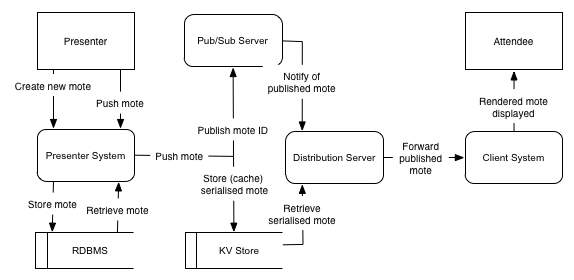
\includegraphics[width=1\textwidth]{dfd}
\end{figure}

\subsection{Presenter System}
The presenter system was designed as a web application using the Django framework, using an interpretation of the MVC design pattern, referred to by the designers of Django as the `MTV' pattern (Model, Template, View). This pattern defines `model' the same way as in MVC, as the definition and structure of system data, `view' as `which data is presented' and `template' as `how the data is presented'\cite{djangomvcfaq:web}.

Implementing the presenter system as a native, `desktop', non-web-based application was also considered. However, it is more likely that a presenter will have access to a browser than the ability to install and configure software on systems. The author also has more experience developing web based applications than native applications, and felt the simple database interactions planned would be more suited to a web-based system.

The presenter system was designed to be the primary system for managing and storing motes and plans, it was therefore necessary to establish an idea of the models which would be used for each. Figure \ref{fig:classdiagram} shows the initial basic model structure concept.

\begin{figure}
\caption{Original concept model diagram}
\label{fig:classdiagram}
\centering
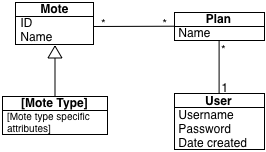
\includegraphics[width=200pt]{classdiagram}
\end{figure}

A base `Mote' model serves as the central model around which the whole system is designed. This base Mote model would only contain Name and ID attributes (as they would be the only common attribute between all motes), as well as some utility methods. Mote types derive from this model, adding their own fields where required. This polymorphic design, combined with Django's concept of `apps' both aid with the requirement to create a modular, extensible system.

Also considered was implementing a more abstract way of defining and extending content types, perhaps using an EAV (Entity-attribute-value) database model. This would reduce the need for developers to write code to add new types. However, this would also mean creating a framework for automatically generating code for the client representation and feedback representation, so it was felt that this would complicate the project beyond its scope.

A Plan model would be used with a many-to-many relationship to the base Mote type, allowing it to refer to a list of any combination of mote types, using polymorphism to retrieve their full attributes when required. The Plan model would also `belong', through a one-to-many relationship, to a User, modelled by a username, password and date created. During development, the User model was implemented by Django's built-in `auth' application, so the final implementation included a number of fields which were not initially planned.

The presenter system required the ability to add, edit and delete both motes and plans. Opting to use Django's built-in generic views, with additions where necessary, would reduce both the design and implementation work needed to create these basic operations.

\subsubsection{Modularity and the Mote Model}
The Django 'app' concept allows sections of the system to be separated in to individual modules, with their own models, views, resources and templates. To support modularity in Diffuse, new mote types are created in separate Django apps containing a model which extends the `Mote' model, implements a serialisation method on the new model, and defines how the mote should be represented on the client and the presenter systems. Motes are all treated as their base class, specialised when additional mote-type specific data is required through the use of django-polymorphic\cite{djangopolymorphic:web}

Developers wishing to extend the system need only add a new app to the presenter system and the entire system will now take advantage of it - this should be the only place in the system where content types need to be defined - the distribution and client system should not need to be updated. 

The Mote model was designed to use three methods, all of which are used to communicate with the distribution server:
\begin{description}
\item[as\_dict] \hfill \\
Returns a Python dictionary of model instance attributes and metadata. Derived classes override this method in order to add their own data to the dictionary. This is used to build a JSON representation of the model instance to be sent to the distribution server.
\item[cache] \hfill \\
Cache uses the redis-py\cite{redispy:web} library to store the JSON representation of the mote in Redis, making it available at the key: ``mote:{[}mote\_pk{]}''. This uses the as\_dict method and does typically not need overriding by derived classes.
\item[push] \hfill \\
Uses redis-py to publish a message to the Redis pub/sub channel specified by a parameter to the method. The message contains the event string and some data, in this case, the event `adminPublishedMote' and the ID of the mote. It   sets a key `plan:{[}plan\_id{]}:latest\_mote' to the ID of the latest mote, so that clients that aren't currently subscribed to the plan's channel can find the latest mote when they choose to subscribe.
\end{description}

JSON was chosen for mote serialisation as both Python and JavaScript have native support for it, it is also very lightweight, designed for data interchange between web applications where there is no need for additional context to be present in the serialised data. Alternative forms of serialisation, including XML and `pickling' in Python. XML were considered too heavyweight, containing a lot of context data which was not required - it was also found more difficult to parse. Language-dependent serialisation methods such as pickling would have been another alternative, but would be hard to decode cross-language.

\textbf{Also considered:}
\begin{itemize}
\item The original design had the presenter system send a post HTTP request directly to the distribution server when a mote was pushed. A version of Redis was released during development which implemented its own Pub/Sub protocol so this was switched to in order to simplify and speed up communication.
\end{itemize}

\subsubsection{The User Interface}
The presenter user interface was not planned or designed before development, it was considered that this method often creates interfaces that have had elements `tacked on' to suit changing features and can often be hard to use due to a lack of understanding of how the system works. While building the system, it becomes evident where elements make the most sense, so creating the UI was an evolutionary process that was not considered fully `designed' until the end of the last iteration.

One of the primary goals for the user interface during its evolution was to ensure it was simple and easy-to-use. This was achieved by a decision to reduce all operations down to two modes of interaction:
\begin{description}
\item[Lists] \hfill \\
Lists are used to represent available plans and motes. Lists are always present in the first two columns of the interface. Three actions are possible on lists and list items:
\begin{description}
\item[Selecting] \hfill \\
In the case of plans, this displays the motes within that plan, for motes, this broadcasts the mote.
\item[Editing/Deleting] \hfill \\
These options are presented modally on hovering over the list item. Editing takes the user to the second type of interaction, 'forms', while deleting prompts the user to permanently remove the item.
\item[Adding] \hfill \\
At the bottom of a list, there is usually a way to add a new item to that list. The item created is always the same as the type of item in the list - the add button at the bottom of a plan list will always create a new plan.
\end{description}
\item[Forms] \hfill \\
Forms modify attributes on items - while they can contain different fields, they all take the same structure whether the user is adding or editing an item. Editing items displays the same form as adding an item, only with fields pre-populated. Forms are only ever shown in the last column of the interface.
\end{description}

\subsubsection{Rendering Feedback}
The final part of the presenter system is how feedback from clients is displayed to the presenter. When a mote is pushed, the last column updates with some representation of received data - how this data is displayed is specified by the individual mote applications, and can therefore vary between mote types.

The original design for implementing feedback rendering was to use HTML templates, as with the rest of the system, however, during their implementation in the interactivity iteration (iteration 4), it was noted that all the templates were very similar; a container which had content injected by JavaScript. It was therefore decided to do away with the template system and implement them entirely in JavaScript.

The new design had individual mote types specify a JavaScript file in the motes' app containing a class derived from Renderer. A set of events are bound to the active Renderer, which call methods on the class when they are triggered. Each method\footnote{Note that methods in JavaScript typically use camel case for method names, whereas in Python, PEP8 dictates that methods should be all lowercase, with underscores separating words} needs to be overwritten by the derived, mote type-specific class:
\begin{description}
\item[render] \hfill \\
Builds the relevant representation of the results within the container with the `renderer' ID. This is called when the renderer is first initialised.
\item[redraw] \hfill \\
Updates the representation with any new data received.
\item[updateData] \hfill \\
Updates the renderers' set of responses with any new responses passed to the method, if the 'append' parameter is true, responses are added to the existing set. If it is false, responses are cleared before new ones are added.
\item[clientDisconnected] \hfill \\
When the client disconnect event is fired, the renderer may choose to remove that clients' response from the display, this method is used to achieve this.
\end{description}

An example implementation of a renderer is that used for the \emph{Question and Answer} mote type. For this, the render method creates a column chart using the HighCharts\cite{highcharts:web} library. the updateData method directly modifies data in the object created by HighCharts, rather than drawing a new chart every time - this created a smooth `sliding' effect on the chart as new data arrived.

\subsection{Distribution Server}
As this system is intended for use in large organisations, such as universities, it is likely that there will be thousands of clients attempting to request motes simultaneously. Combined with the need to maintain a persistent connection to each client for broadcasting content and provide updates within a short time, it was felt that a traditional server would not be suitable, so the distribution server was introduced.

\subsubsection{Dealing with Scale}
The concern with broadcasting content in real-time to hundreds of devices at a time using a typical web server was that it is likely to struggle with the number of requests. Techniques used to emulate real-time communication either require a permanent connection open to the server, or hundreds of requests to the server per minute. Traditional web servers such as Apache use a process-based model, where each additional request requires a new thread meaning many hundreds of connections being opened and closed per minute not only causing high memory usage, but incurring quite a large processing overhead, increasing the time it takes to serve a request as the volume increases.

An event-based server was chosen as the solution to this issue, which use a single thread and an event loop, removing the requirement for context switching. While this does mean significantly lower memory usage and overhead, it doesn't prevent operations in code from blocking, particularly those that involve I/O. For example; a request which queries the database will temporarily hold up the loop until the database responds, as we require a very quick response from the server, this may prove unacceptable.

To solve this, a distribution server was designed in an event driven programming language, which work in the same way as an event driven server - using a main event loop to support callbacks from functions so that operations can continue while I/O is being performed, operating on the results only when they return.

This type of programming paradigm is implementable in the majority of programming languages, although it is more prevalent and easier to implement in functional languages such as Erlang and Scala. There are also a number of frameworks for other languages available which support event-driven networking, such as Twisted (for Python), EventMachine (for Ruby) and Node.js (for JavaScript). 

As the author was not familiar with functional languages, implementing a server in Erlang or Scala was not attempted, but instead existing event-driven networking frameworks were researched as they did not require learning a new language and seemed relatively popular. Twisted and EventMachine are mature frameworks, both with a large community and many extensions, but they both seemed too bloated for what was needed. Node.js is a relatively new framework which is rapidly gaining popularity, primarily because of its speed and simplicity - it was particularly interesting due to its use of JavaScript which is also used by the client system (an opportunity for more code reuse and resource sharing) and is a language with which the author was familiar. It is also designed to be exceptionally easy to use to write a simple server.

Using the event based constructs in Node.js, a server was designed tailored to the type of communication needed, thus tackling the blocking I/O problem on two fronts; reducing the amount of I/O time required through caching, and attempting to prevent I/O from blocking. To cache, the presenter system pushes serialised versions of motes to Redis and uses the distribution system to quickly retrieve and push these out to clients.

\subsubsection{Distributing the Motes}
As this application required content to appear on all client devices within a reasonable period of time after they are broadcast, it needed to use some form of real-time communication method. As both the client and presenter are web-based, choices for doing so are quite limited due to the HTTP protocol being entirely request-response oriented. If code which was not being executed in the browser was used, it would be possible to use networking technologies such as sockets to allow the client to 'listen' for communication from the broadcaster.

However, there are various ways to support a  communication channel in web applications:
\begin{description}
\item[WebSockets] \hfill \\
An implementation of a communication channel over TCP for use implementation in web browsers as part of the W3C HTML5 specification. Currently only implemented in the latest version of modern browsers, excluding Internet Explorer.
\item[Flash Sockets] \hfill \\
TCP sockets can also be implemented using the ActionScript 3.0 Socket class, requiring the browser to load a Flash file and therefore requiring the Flash browser plugin. While this is the next best thing to using WebSockets, many mobile browsers do not fully support Flash.
\item[Ajax long polling] \hfill \\
A technique which is most commonly used for real-time web applications as it only requires a browser to support the XMLHttpRequest object, commonly used for Ajax interactions. This technique makes an asynchronous request to the server which the server keeps open until it has new data to send. As soon as new data has been received, the browser starts a new long polling request. While this technique is available on more devices, it is also slower and causes the browser to constantly be in a 'loading' state.
\item[Multipart streaming] \hfill \\
The XMLHttpRequest object can also be used to react to a server using a multipart content type; suggesting to the browser that the response will be delivered in multiple parts. The browser keeps the connection open and calls a callback function whenever a new part of the response is delivered.
\end{description}

Unfortunately, the only one which reliably works on a large subset of browsers is long polling. The system could have been implemented using just this techniques, but it would then be unable to take advantage of the faster protocols such as WebSockets, available on the latest mobile browsers (such as Safari on iOS 4.2.1).

To save writing implementations of each communication method, A library available for Node.js, socket.io\cite{socketio:web} was chosen, which allows the client and server to determine which communication technique to use depending on what they each support. It provides a simple API to abstract these techniques away and allowed me to simply request some data be transmitted. 

\subsubsection{Server Design}
The design of the server was largely based around the use of the Connect middleware framework for Node.js. Connect creates a basic HTTP server, with middleware for serving static files (used to serve the client application) and for session management.

On top of the basic HTTP server, an event-based cross-system communication micro-protocol was designed. A typical communication would be a JSON string containing two top-level objects: `event' and `data'. The former contains a single camel-cased string describing the event which triggered the communication. The latter contains all the relevant data pertaining to the operation.

Operations were intended to be triggered by events from the Pub/Sub channel and from the connected sockets. For example, when the event  with the event string `adminPublishedMote' was published on the Pub/Sub channel, a function would be called which parses a `data` object and forwards the parsed mote to clients connected to the server and subscribed to the relevant plan.

Along with supporting communication through the socket one way (pushing motes out to clients), the server also needed to deal with responses coming back from clients. To do this, it would listen for the `clientRespondedToMote' event on the socket and store the answer in a plan/mote specific hash in Redis.

Whenever the distribution server needs data, it is requested from Redis using the node\_redis\cite{noderedis:web} library. Redis, being very efficient at retrieving data by key from memory (a time complexity of O(1)) required very little time to fetch the required data (although even then, due to the event-loop nature of the server, it continued processing requests).

Redis was used heavily in the design to reduce the amount of I/O needed to store and retrieve data on the server. Rather than requesting data from the presenter server when it was needed (triggering a request to the RDBMS or filesystem), the presenter was designed to cache any relevant data in Redis before the distribution server needed it. This included serialised motes, mappings between plan `access codes' and plan IDs as well as the current status of plans.

Due to the design changes made to client authentication so that the system does not request a user be logged in on the client to respond to motes, it is necessary to make some assurances that a single device is a single user. To do this, Connect's session management middleware combined with the Connect Redis\cite{connectredis:web} session backend to store user sessions in Redis was used to maintain sessions. Session keys are used throughout the system as a unique user identifier, so when a user refreshes Flux, rather than creating a new response, their old response is overwritten.

Using sessions also allows a `clientDisconnected' event to be fired when the session expires (when the user no longer has Flux open). The server then removes that users' response and notifies the presenter, which will in turn call the `client\_disconnected' method on the currently active renderer, removing their answer in realtime.

Initially, there was no design or convention for the naming and structure of keys in Redis. During development, it was found that attempting to get/set various keys in multiple places in the application was confusing and hard to follow without a basic design. This lead to the documentation of an outline structure of keys:

\begin{tabular}{ l p{290pt} }
  \textbf{Key Structure} & \textbf{Intended Value} \\ \hline
  \textbf{mote:[mote\_id]} & Basic string value containing full JSON for mote with ID of [mote\_id] \\
  \textbf{plan:[plan\_id]:mote:[mote\_id]} & Hash value containing all client responses to [mote\_id] subscribed to [plan\_id], hashed by client ID. \\
  \textbf{plan:[plan\_id]:latest\_mote} & ID of latest mote on [plan\_id] \\
  \textbf{plan:[plan\_id]:name} & Full human-readable name of [plan\_id] \\
  \textbf{plan:[plan\_access\_code]} & ID of plan with access code of [plan\_access\_code] \\
\end{tabular}

Rather than using a separate key-value store, caching serialised motes directly in memory on the distribution server was also considered. However, it was felt that if the system were serving thousands of clients at a time, using a key-value store designed for this type of storage would be more suitable. There were also a number of benefits of using a separate store, particularly that multiple systems could communicate directly with it and that it would be simpler to maintain as a separate entity.

\subsection{Client System}
The client system is a critical component for meeting the requirements of the project. Referred to as Flux, this is the system which attendees connect to in order to receive broadcasted content.
While the resources (HTML pages, JavaScript, etc.) for this component are designed to be served both from the distribution server and the presenter system, it is considered a separate entity as the majority of its operations are on the client-side, in JavaScript.

\subsubsection{Why web-based?}
In platform research, it was noted that every platform studied had a proficient browser, most being based on the WebKit\cite{webkit:web} open source project (providing HTML rendering and JavaScript implementations) which is also used for Google's Chrome and Apple's Safari browsers. From past experience, the author knew how web applications can be used for excellent cross-platform support, backed up by research in to existing multi-platform ARS' systems, which all appear to be web-based. 

A web-based client would be accessible from any device with a browser that supported full HTML, JavaScript and some form of real-time communication protocol (even if emulated), features which all of the devices researched have. No device-specific code is required, although styles for different screen sizes are necessary. It is also possible to use technologies only present in more modern browsers (such as HTML5 features) by making use of graceful degradation on devices that do not support it.

Therefore, a browser-based solution for the client was chosen as it was felt that it was the most appropriate option for a truly multi-platform system. While some of the flexibility of device-native applications may have been lost, this was considered an appropriate compromise. The author's past experience with web applications using JavaScript and an understanding of how to implement a real-time application also contribute to this decision.

A number of alternative options were researched, including common libraries, cross-platform libraries and rich multimedia platforms. A brief discussion on these can be found in Appendix \ref{app:implementationoptions}.

\subsubsection{System Design}
On loading, Flux attempts to connect to the distribution server using the client-side version of the socket.io library. This establishes a realtime method through which to communicate for the rest of the session. The same event-based micro-protocol was used here in order to deal with events from the distribution server. For example, receiving a communication with the event `serverPushedMote' triggers a function which updates the display. These two features combine to create a simple web page which updates in realtime, on request.

In order to render a pushed mote, Flux performs a variety of operations triggered by its update\_mote function. It begins by updating the list of past motes available in the history panel. It then attempts to load the scripts and styles required by that mote type. This is done by using yepnope.js\cite{yepnope:web} to check whether the scripts are already loaded, and if not, request them from the distribution server. The distribution server proxies to the motes' resources the developer created for the presenter system and returns them Flux.

Once these resources are loaded, the returned JavaScript resource will contain a subclass of ClientMoteRenderer (named after the object identifier) which is instantiated and has its `render' method called. This method fetches the mote types' template (again, created by the mote type's developer) which will be written using the mustache\cite{mustache:web} template language and rendered using mustache.js\cite{mustachejs:web}. The ClientMoteRenderer subclass will likely implement additional functionality which will eventually trigger Flux's `respond' function, returning the users' response to the distribution server.

For example, QaRenderer, the implementation of ClientMoteRenderer which is loaded when a mote of type Question and Answer is pushed calls the respond function with the answer the user has selected and updates the display to show some feedback to the user.

\todo[inline]{Also considered?}

\subsubsection{User Interface}
It was important that this part of the system was very easy to use. One of the ways this was achieved was by limiting the amount of choices a user had at any one point. On initially loading the system, they user is prompted to enter the access code for the plan they wish to join. This is the only option they have available at this point. Entering the code will trigger a communication with the distribution server to check whether the access code matches an existing plan. If it does, the page will be updated with the most recently pushed mote to that plan.

The renderers implemented for the built-in mote types are designed to respond immediately on interaction - there is never a need to select a `send' button so that the user never needs to understand the concept of communication between client and server.

There are two other interface elements available to the user, neither of which are critical to its operation. The first, visible to the top left, is the currently active plan. Selecting this will allow the user to change to another plan. The second, available to the top right, is a history panel. Selecting this will drop down a list of all past motes, allowing the user to navigate back to a previous mote if desired.

\subsection{Mote Types}
A number of mote types were designed to demonstrate the system, each for a different type of interaction and use. The only mote type initially designed was Question and Answer, the rest being designed in later iterations once the majority of functionality was in place.

\subsubsection{Slide}
The Slide is the most basic mote type available in Diffuse, created to demonstrate the basic ability to push non-interactive HTML content to Flux.

When creating a Slide, the presenter is prompted to complete a `Content' field in which they can enter any HTML content for the slide. The administrator interface implements the TinyMCE\cite{tinymce:web} WYSIWYG editor with django-tinymce\cite{djangotinymce:web} to allow the presenter to generate HTML by using a simple editor.

When pushed to Flux, this mote type simply re-renders all the HTML defined by the presenter.

Uses of this mote type include:
\begin{itemize}
\item As title/divider content - if Diffuse is being used as the primary form of presentation, title motes can be pushed to users.
\item Instructive content - for displaying instructions to the attendees.
\item For content which requires physical interaction. For example, a presenter might still want to encourage the raising of hands.
\item Content shown only to a subset of attendees. The presenter might be interested in dividing the group into multiple subgroups, each with their own plan and access code. The presenter could then broadcast some informational content to a subgroup without letting the other groups see it.
\end{itemize}

\subsubsection{Question and Answer}
The Question and Answer mote type was created to show a basic, immediate response type of interaction and as a direct comparison to the questions content that standard ARS systems are primarily used for. It defines a `Question' model derived from Mote, as well as an `Answer' model with a many-to-one relation between answers and questions.

Creating a Question and Answer mote requires the following fields to be completed:
\begin{description}
\item[Question Text] The question shown to the attendees.
\item[Answers] A list of answers with a text string, and an option to select whether the answer is considered `correct' or not.
\end{description}

This mote type is presented on Flux as a question with a list of answers. Selected answers are highlighted and immediately pushed back to the distribution server.

Answers are shown to the presenter in the form of a column graph (using HighCharts) showing the number of attendees that responded with each answer. As new answers arrive, this graph updates in real-time with the new respondent's answer. The graph's scale changes automatically if numbers begin to move off the original scale. Should a user change their answer or disconnect, their previous answer is dynamically removed from the graph and replaced with their new one (if they submitted one).

Answers marked as correct are shown on the response graph as a green bar. Although this option is not used for any other feedback, it is used to demonstrate how attributes can affect how motes are displayed.

Uses of this mote type include:
\begin{itemize}
\item Prompting attendees for feedback from a set list of answers (Enjoyed, did not enjoy, etc.). 
\item Asking a question related to materials discussed in the presentation. Useful in a lecture for understanding how well students understand the material, allowing the presenter to rapidly know what they need to explain in more detail, etc.
\item As an anonymous alternative to `hands up' situations, where attendees are prompted to select some relatively private information (such as what category they fall into) without having to alert all other attendees.
\end{itemize}

\subsubsection{Association}
The Association type demonstrates a more `puzzle' type of question, showing the potential flexibility available for creating feedback mechanisms. The type defines an `AssociationGroup' model derived from Mote, along with an `Association' model with a many-to-one relation between associations and association groups. 

An association is defined as two strings, the left side, and the right side. When presented to a client, both the left side and right side are randomised separately, prompting the user to 'join up' the left side with its original right side. This is done by dragging a line between the two columns. The line drawing effect was implemented using Raphael.js\cite{raphaeljs:web} for drawing lines between boxes, and making use of the jQuery UI for iPhone, iPad and iPod Touch\cite{jqueryuiipad:web} plugin to allow map jQuery's dragging events to their equivalent touch events (so that dragging would work correctly on touch devices).

To demonstrate possibilities for delayed response, the client only submits the users' answers once the user has attempted to match all associations. The mote type is shown to the presenter as a  HighCharts pie chart, displaying segments for the number of correct answers submitted. For example, a `4' segment would be displayed showing the percentage of users who correctly matched four associations. This is dynamically populated with the number of associations possible. A question with 20 possible associations will automatically generate a graph with 20 possible segments.

The primary use of this mote type is to prompt users to match two sets of related data - countries to capitals, equations to correct answers, etc.

\subsubsection{Heatmap}
The Heatmap type was created to demonstrate interactions with different types of media, in this case, images. It defines a simple `Heatmap' model, extending Mote which contains an attribute for an image, Django and PIL\cite{pil:web} (Python Imaging Library} handle the image upload and storage operations. 

When pushed to Flux, the full image is shown to the client. On clicking/touching the image, a small marker shows where they have selected. The presenter sees the same image in the presenter interface with the addition of a heatmap overlay, showing areas with low click density in yellows and greens, up to those with higher click density in oranges and reds. The heatmap code was based off the work of Patrick Wied\cite{heatmap:web}.

Uses of this mote type include:
\begin{itemize}
\item Showing a screenshot, graphic or photograph and prompting the users to point out a certain feature/error on the image.
\item Displaying a map and prompting users to select where they live, giving the presenter an idea of the geographical distribution of the attendees.
\item As a more complex Question/Answer type, by presenting a graphic with multiple options and asking attendees to touch the correct answer.
\end{itemize}

\subsubsection{Feedback}
Feedback motes demonstrate a more complex interaction between attendees and the presenter, making use of a text field to prompt for any string of text. It is defined by a simple`Feedback` model which only defines a `description' attribute. 

When pushed to a client, the description attribute is displayed along with a text entry form. Whenever the text entry form receives input, this is immediately returned to the distribution server.

The presenter interface is a live-updating list of all text entry fields from users - the presenter will see every user typing in real-time on their display. If a user removes all text from their entry field, this entry is also completely removed from the presenter interface. To reduce network load, changes to the client entry field are only checked and returned every 250ms (through the use of the jQuery Throttle\cite{jquerythrottle:web} snippet).

Uses of this mote type include:
\begin{itemize}
\item Prompting the attendees for any questions they may wish to ask. While not intended to replace asking out loud, presenters may prefer this option as they are given the option to browse a list of questions for ones they consider important. It also gives attendees who may not wish to speak in front of a crowd the option to ask questions.
\item Prompting attendees for presentation feedback or comments.
\item Asking for the answer to a question which may not have a defined set of answers, or where preset answers are not appropriate.
\end{itemize}

\pagebreak
\section{Problems}
\subsection{Communication protocol}
Once the distribution server was communicating in both directions with the client, the issue of making communications trigger operations on each system arised. There were issues with figuring out a way to establish a light RPC protocol, until inspiration came from the nodechat.js\cite{nodechatjs:web} which used an event based model, including an event string as part of the communication between systems. 

Implementing this was simple, and it made the system much more flexible, however, the triggered events were not fully designed before implementing them, so it was often confusing to figure out what was triggering which events, when to respond to them, and how to `bubble' them through all three systems when required. To resolve this, a naming convention was established for events; starting with the system from which they originated; `admin', `server', `client', followed by the operation which triggered the event (rather than the operation the event should trigger) in the past tense. 

For example, the `clientRespondedToMote' event is triggered by the client when the user responds to a mote. This event is returned to the admin by triggering the `serverPushedResponse' event.

The other issue experienced with this protocol was maintaing context between communications. For example, if the client requested the existence of a plan from the distribution server, it was necessary for the distribution server to know which client requested it, and the client needed to know when it received a response. 

As there would be no concept of a `response' to a certain communication in this protocol, there were issues figuring out how to know when the distribution server was responding. The eventual solution to this was to include just enough context in the sent message so that the response could be identified and to remove the need for context from events. For example, the client identifier would be sent with the request for the existence of a plan so that the distribution server could trigger a `serverSetPlan' event only on the requesting client.
 
 \subsection{Dynamic resource loading}
One of the more complicated issues which arised when developing Flux was the issue of dynamically loading mote-type specific resources on request. 

The first issue encountered with this was a race condition where the system would attempt to instantiate the mote's ClientMoteRenderer object before it had successfully loaded. A fix was attempted by instantiating the object in a callback triggered by the resource loader, but the race condition still existed when the resource had loaded but the browser had not fully interpreted the new script. Eventually this was fixed by using yepnope.js, a script loader which had built in callback functions which worked perfectly.

The second issue with this was with maintaining mote type modularity. Originally, all mote-specific resources for Flux were stored in a separate directory from the main mote type definition, this allowed the distribution server to be used to serve these resources. However, to meet flexibility objectives, it was desired that all mote-specific items be in a single folder, regardless of whether they were used for Diffuse or Flux. To achieve this, these resources were moved in to the folder which would typically be served by Django and updated Flux to find them on the Diffuse domain. 

However, because the client was being served from the Flux domain, and JavaScript resources were attempting to load from another domain, the same origin policy implemented in most browsers prevented them from loading. An attempted work around was to request the JavaScript resource using JSONP, but this added extra unnecessary complexity. The final solution was to use Nginx to proxy requests for the resources on the Flux domain to the Diffuse resource folder.

\todo[inline]{More problems - perhaps saving error when demoing?}

\pagebreak
\section{Testing}
A number of testing strategies were adopted during the development of the project, each serving a different purpose.

\subsection{Testing during development}
An informal testing strategy was used during development cycles. This usually consisted of
\begin{itemize}
\item Creating a `test' entries in the presenter system database and ensuring they worked as the system was built. 
\item Adding debug code (logging, prints, debug output) to systems.
\end{itemize}

The use of Django's fixtures system made it easy to load a set of test data in to the database during development. Combined with the use of South\cite{south:web} to create data migrations when models were changed, persistent test data was a valuable way to ensure the system was working.

This approach was used primarily to the workings of the system could be clearly seen as it was built. It was not intended to ensure the system met specifications.

\todo[inline]{Expand if possible}

\subsection{Iteration Testing}
At the end of every iteration, a testing plan was executed to ensure that what was built met the specifications determined at the start of the iteration. Feedback from this testing then went in to planning the next iteration.

\todo[inline]{Expand if possible, refer appendices}
\todo[inline]{Create appendices for testing}

\subsection{Automated Stress Testing}
As this system is built around many clients connected simultaneously, it was necessary to test how the system would behave under normal use. As only a few client systems at a time were available, a set of scripts were wrote to emulate the behaviour of clients in order to ensure that the distribution system and presenter system renderers could cope with normal (and abnormal) numbers of responses.
\todo[inline]{Expand if possible}

\pagebreak
\section{Evaluation}
The system was successful in improving on the three areas defined in the objectives:

\subsection{Accessibility}
\subsubsection{Improving ease and cost of setup/configuration}
By implementing the system entirely in software and supporting communication over existing networks, the project successfully improves on ease and cost of setup/configuration for system administrators. There is no additional configuration required for individual presentations, so as desired, the system only requires configuring once.

However, the system is dependent on a large number of tools and libraries. Configuring these as the author has done in another environment is likely to be complicated and error-prone. If the system were to be distributed, it would likely need to be reconfigured to reduce external dependencies and distributed as some form of `package'. There is also a number of areas of the system where some configuration variables are hard-coded (such as domains); this would need to be addressed by separating all of these variables out to configuration files.

The communication of system services entirely over web-based services means there is no need for additional firewall configuration as long as HTTP traffic is allowed around the network. Support for WebSockets does not require any additional ports due to HTTP's UPGRADE method. 

A potential shortcoming in system communication is between the presenter system and the distribution server. This requires a shared Redis instance accessible by both systems so that the presenter system can publish to the pub/sub channel. This would require either the presenter system, the distribution server and the Redis instance to be on the same machine (presenting potential scalability issues), or requiring additional firewall configurations to allow the Redis instance to be accessed over the network (presenting potential security issues). This could have been avoided by having the presenter system publish content to the distribution server over the established socket, or over HTTP.

\subsubsection{Facilitating ease of access by presenters}
As specified in the system objectives, there is no requirement to install additional software on individual systems. Presenters are able to access a URL on the network in a browser for access to the presenter system. 

An issue with this approach is that the presenter system is not fully operational on all browsers. Due to time constraints, it was only tested in modern browsers such as Mozilla Firefox and Google Chrome and uses features of CSS3 and HTML5 which are not supported in many versions of Internet Explorer. Considering a number of businesses do not support modern browsers, this could potentially be an issue for them. However, considering the focus of the project was the way in which these systems communicate, optimising for old browsers would have been time better spent elsewhere.

\todo[inline]{logging in?}

\subsubsection{Supporting existing devices}
\label{sec:supportexistingdevices}
The Flux web client, while optimised for iPad, has been tested and runs well on iPhone, Android phones and most modern browsers (again, Chrome and Firefox). While this does meet the requirement that it runs on existing mobile devices, it was not tested on a large number of the platforms initially researched (Windows Mobile, Windows Phone 7, BlackBerry OS and Symbian) due to the authors' limited access to devices using these platforms. 

However, should these devices not function correctly, the system was designed to allow for modifications to the client without affecting the rest of the system due to the low coupling between mote type definitions, Flux, and the presenter system. Modifying individual mote type JavaScript to include feature detection or bug fixes for certain platforms would be relatively easy and would not require restarting the server.

The flexibility offered by allowing the developer full access to the JavaScript used by each mote type could be an issue as it is possible that they will implement features not supported by some user agents. For example, one of the demonstration mote types, Association, requires the browser to support SVG, which is not supported in Android devices. If the developer of this mote type did not create some form of fallback, this mote type would not work correctly on these devices. 

The solution to this would be to create a more limited subset of fully tested features which developers could implement in their mote types through a defined API. Implementing this would have involved designing, developing and documenting this API, which would have been time consuming and could be considered outside the scope of the project. It would also mean significantly less flexibility afforded to developers creating mote types.

\subsubsection{Removing dedicated hardware requirement}
There is no dedicated hardware required for using Diffuse, meeting the objectives specified for the project. The two servers can be configured on existing hardware, communication is designed to work over the existing network, and clients do not require proprietary `handsets' to interact with the system - they are able to use their own mobile, portable or desktop devices.

Should an establishment not have an existing network infrastructure, there would be significant costs and work required to set one up in order to use Diffuse. It is likely that there would be no incentive to configure a network solely to use Diffuse, but for smaller establishments, it is conceivable that the Diffuse servers could be configured on a single desktop PC with a wireless router attached and still be highly functional.

There is also the issue of the prevalence of devices which would run the client. While in some establishments it is likely that the vast majority of attendees are likely to have a compatible phone or laptop, in others those attendees might be in the minority. Supplying all other users with a suitable device may be more expensive to the presenter than purchasing dedicated ARS hardware. Considering the problems Diffuse attempts to solve, this issue is unfortunately unavoidable, however, it is hoped that this system will be attractive to those establishments where attendees are likely to own these devices and will value the improved interactivity provided by Diffuse.
\todo[inline]{More research?}

\subsubsection{Simplifying interaction experience}
Interaction with the client system is improved in Diffuse over typical ARS' through the use of a graphical interface. Being able to click or touch items/answers directly without the user having to deal with the abstract concept of matching answer numbers/letters with a slide on a different screen, or pressing `send' buttons to respond makes the system much more intuitive to use. Being able to use a full colour screen also allows additional instructions and guidance to be presented to the user where required.

Presenting all the information required on screen on the users' own device also makes this system valuable for disabled users, for example, blind users using an iPad with VoiceOver enabled will be able to have the question and answers read to them. This benefit is unfortunately limited to some mote types, as VoiceOver will not be as valuable to the blind user with images, or drag-and-drop puzzles. It is left up to the presenter when each type of content should be used.

An issue with this is the lack of tactile feedback from screens - there is no physical response to pressing a button, so a user may have issues with knowing when they have correctly submitted a response. To alleviate this, visual cues such as highlighting are used to show a user what options they have selected.

The presenter interface is designed to be simple and easy-to-use. During informal testing, testers found it simple and were able to create and broadcast plans and motes without any instruction. Many existing ARS' integrated with PowerPoint to create content matched with slides - these often involve a plugin used for turning slides in to questions. This type of use might be more familiar to those used to PowerPoint, to whom Diffuse may be initially confusing. There are also likely to be those who do not like the idea of creating two sets of content, one for presentation and one for interaction.

\subsection{Interaction}
By leveraging the flexibility of the web browser found in targeted devices, Diffuse is able to offer a large variety of types of interaction. From simple Question and Answer interactions found in standard ARS systems, through complex puzzle-like association questions, to interactive images.

\todo[inline]{Lots of examples of potential uses}

\subsection{Flexibility}
Developing the system around a modular framework from the start meant the final version of Diffuse is very flexible and extendable. All final mote types were written after the main system was developed without any additional changes needed to the core system. This demonstrated that any developer with knowledge of the workings of the system could create almost any type of mote type they required.

Apart from the issues this flexibility causes with device compatibility detailed in section \ref{sec:supportexistingdevices}, there are also a few shortcomings with the implementation. Primarily, in order to set up a new mote type, the system administrator must run a few Django administration commands in order to generate the correct database tables. While these commands are relatively simple and require very little learning, this is an awkward step which could be alleviated by creating some form of plugin framework which allowed the administrator to enable mote types from the administration interface. 

\todo[inline]{Potential for future developments}










\bibliography{bibliography}

\begin{appendices}
\appendixpage
\addappheadtotoc
\section{Project schedule}
\label{app:schedule}
\todo[inline]{Project schedule from progress report}

\section{Report on operating systems}
\label{app:osreport}
\todo[inline]{Report on operating systems}

\section{Implementation options and choices}
\label{app:implementationoptions}
\todo[inline]{Implementation options and choices}

\section{Existing ARS systems}
\label{app:existingars}
\todo[inline]{Existing ARS systems}

\section{Requirements specification}
\label{app:requirements}
\todo[inline]{Requirements specification}

\section{Testing documentation}
\label{app:testing}
\todo[inline]{Testing documentation}
\end{appendices}

\end{document}